\subsection{Trigger}\label{trigger}
\subsubsection{Projektteilbereich Übersicht}
Die Komponente \textit{Trigger} ist wesentlich für die Unterteilung in Pakete. Dieser reagiert auf eine vorgegebene, konfigurierbare Schwellspannung in jedem der drei Modi. Der gewünschte Modus wird vom User-Interface vorgegeben. Einen sogenannten "Single-Shot" kennt diese Komponente nicht, da diese ausschließlich primitiv triggert und sich nicht um "höhere Angelegenheiten" kümmert.
\subsubsection{Funktion}
\paragraph{Modus: Rising Edge}
Bei der \textit{Rising-Edge-Detection} löst der Trigger beim Erreichen und Überschreiten des Schwellwertes (in der Grafik: \textcolor{red}{rot}) aus. Es muss jedoch immer davor, aufgrund der Hysterese, ein vom Schwellwert abhängiger unterer Wert (in der Grafik: \textcolor{blue}{blau}) erreicht werden (arming\_level\_low). Damit wird falsches, zu häufiges Auslösen wegen höherfrequenten und/oder überlagerten Signalen vermieden. Signale mit einer zu kleinen Amplitude ($\leq$ Hysterese) können nicht getriggert werden. In der Grafik \ref{risingEdge} sind 3 Szenarien Abgebildet, nur im ersten löst der Trigger aus.
\begin{figure}[h]
	\begin{center}
		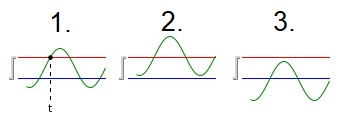
\includegraphics[width=15cm]{SAUER/Grafiken/Trigger/TriggerEdgeRising.jpg}
		\caption{Trigger Rising-Edge-Detection}
		\label{risingEdge}
	\end{center}
\end{figure}
\paragraph{Modus: Falling Edge}
Bei der \textit{Falling-Edge-Detection} löst der Trigger beim Erreichen oder Unterschreiten des Schwellwertes (in der Grafik: \textcolor{red}{rot}) aus. Es muss jedoch immer davor, aufgrund der Hysterese, ein vom Schwellwert abhängiger oberer Wert (in der Grafik: \textcolor{blue}{blau}) erreicht werden (arming\_level\_high). Damit wird falsches, zu häufiges Auslösen wegen höherfrequenten und/oder überlagerten Signalen vermieden. Signale mit einer zu kleinen Amplitude ($\leq$ Hysterese) können nicht getriggert werden. In der Grafik \ref{fallingEdge} sind 3 Szenarien Abgebildet, nur im ersten löst der Trigger aus.
\begin{figure}[h]
	\begin{center}
		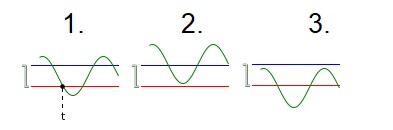
\includegraphics[width=15cm]{SAUER/Grafiken/Trigger/TriggerEdgeFalling.jpg}
		\caption{Trigger Falling-Edge-Detection}
		\label{fallingEdge}
	\end{center}
\end{figure}
\paragraph{Modus: Any Edge}
Bei der \textit{Any-Edge-Detection} löst der Trigger sowohl beim Unterschreiten als auch beim Überschreiten des Schwellwertes (in der Grafik: \textcolor{red}{rot}) aus. Es muss jedoch immer davor, aufgrund der Hysterese, ein vom Schwellwert abhängiger oberer oder unterer Wert (in der Grafik: \textcolor{blue}{blau}) überschritten bzw. unterschritten werden (arming\_level\_high, arming\_level\_low). Damit wird falsches, zu häufiges Auslösen wegen höherfrequenten und/oder überlagerten Signalen vermieden. Signale mit einer zu kleinen Amplitude ($\leq$ Hysterese) können nicht getriggert werden. In der Grafik \ref{anyEdge} sind 4 Szenarien Abgebildet, in der ersten Zeile funktioniert das Triggern, in der zweiten nicht.
\begin{figure}[h]
	\begin{center}
		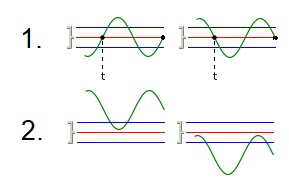
\includegraphics[width=13cm]{SAUER/Grafiken/Trigger/TriggerEdgeAny.jpg}
		\caption{Trigger Any-Edge-Detection}
		\label{anyEdge}
	\end{center}
\end{figure}
\paragraph{Schwellwert, Hysterese und Modi}
Diese Konfigurationseinstellungen werden vom User-Interface vorgegeben. (siehe: \ref{Protokoll}) Für den Schwellwert kann jeder Wert ($\approx$ Spannung) eingestellt werden, jedoch sollte darauf geachtet werden, dass die Hysterese im aktuellen Modus den Wertebereich nicht verlässt. Die Trigger-Unit begrenzt sicherheitshalber die Hysterese dynamisch so, dass diese den Wertebereich nicht verlassen kann.($arming\_level\_low \geq 0, arming\_level\_high \leq 4095$) Der Schwellwert wird nicht in Volt angegeben, sondern im Bereich der Rohdaten des ADCs (0 - 4095).
Eine Hysterese im Bereich von 20 bis 50 digits wird empfohlen.
\subsubsection{VHDL-Design-Unit}
Die Komponente ist sehr einfach gehalten und auch zu bedienen bzw. zu implementieren.

\begin{figure}[h]
	\begin{center}
		
\includegraphics[width=8cm]{SAUER/Grafiken/Trigger/Block.png}
		\caption{Entity Trigger}
	\end{center}
\end{figure}
\begin{center}
\begin{tabular}[h]{|l|l|l|}
	\hline
	Port & Typ & I/0\\
	\hline\hline
	RESET\_n & std\_logic & in\\
	\hline
	CLK & std\_logic & in\\
	\hline
	values\_in\_i & natural & in\\
	\hline
	trigger\_threshold\_i & natural & in\\
	\hline
	trigger\_hyst\_i & natural & in\\
	\hline
	trigger\_mode & trigger\_types & in\\
	\hline
	trigger & std\_logic & out\\
	\hline
\end{tabular}
\end{center}
\subsubsection{Design-Unit Test}
\paragraph{Generelles}
Um die Komponente \textit{Trigger} zu testen wurde eine Testbench geschrieben und mithilfe dieser eine Simulation in ModelSim durchgeführt. Neben der Clock, dem Reset und den Konfigurationseinstellungen wurde als zu triggernder Datenstream ein Dreieckssignal angelegt.
\\Die Design-Unit wurde gut durchgeprüft. Viele Testversuche mit möglichst verschiedenen und auch exotischen Konfigurationseinstellungen ergaben eine fehlerlose Funktionalität. Das Synthetisieren der Komponete stellt ebenfalls kein Problem dar.

\paragraph{Simulation}
Im abgebildeten Zeitdiagramm (Figure \ref{TriggerSim}) ist eine der Simulationen zu sehen. Die Komponente wurde auf den Trigger-Mode \textit{Any} gestellt, was bedeutet, dass sie auf beide Flanken reagiert. Eine Hysterese von 20 digits und ein Schwellwert (=threshold) von 2100 digits wurden eingestellt.\\Es ist zu erkennen, dass die einzelnen, internen Signale aus der Komponente \textit{trigger\_falling} und \textit{trigger\_rising} zum richtigen Zeitpunkt ausgelöst werden. Diese ergeben im Trigger-Mode \textit{any} oder-verknüpft das \textcolor{red}{rot} dargestellte Signal \textit{trigger}. 
\begin{figure}[h]
	\begin{center}
		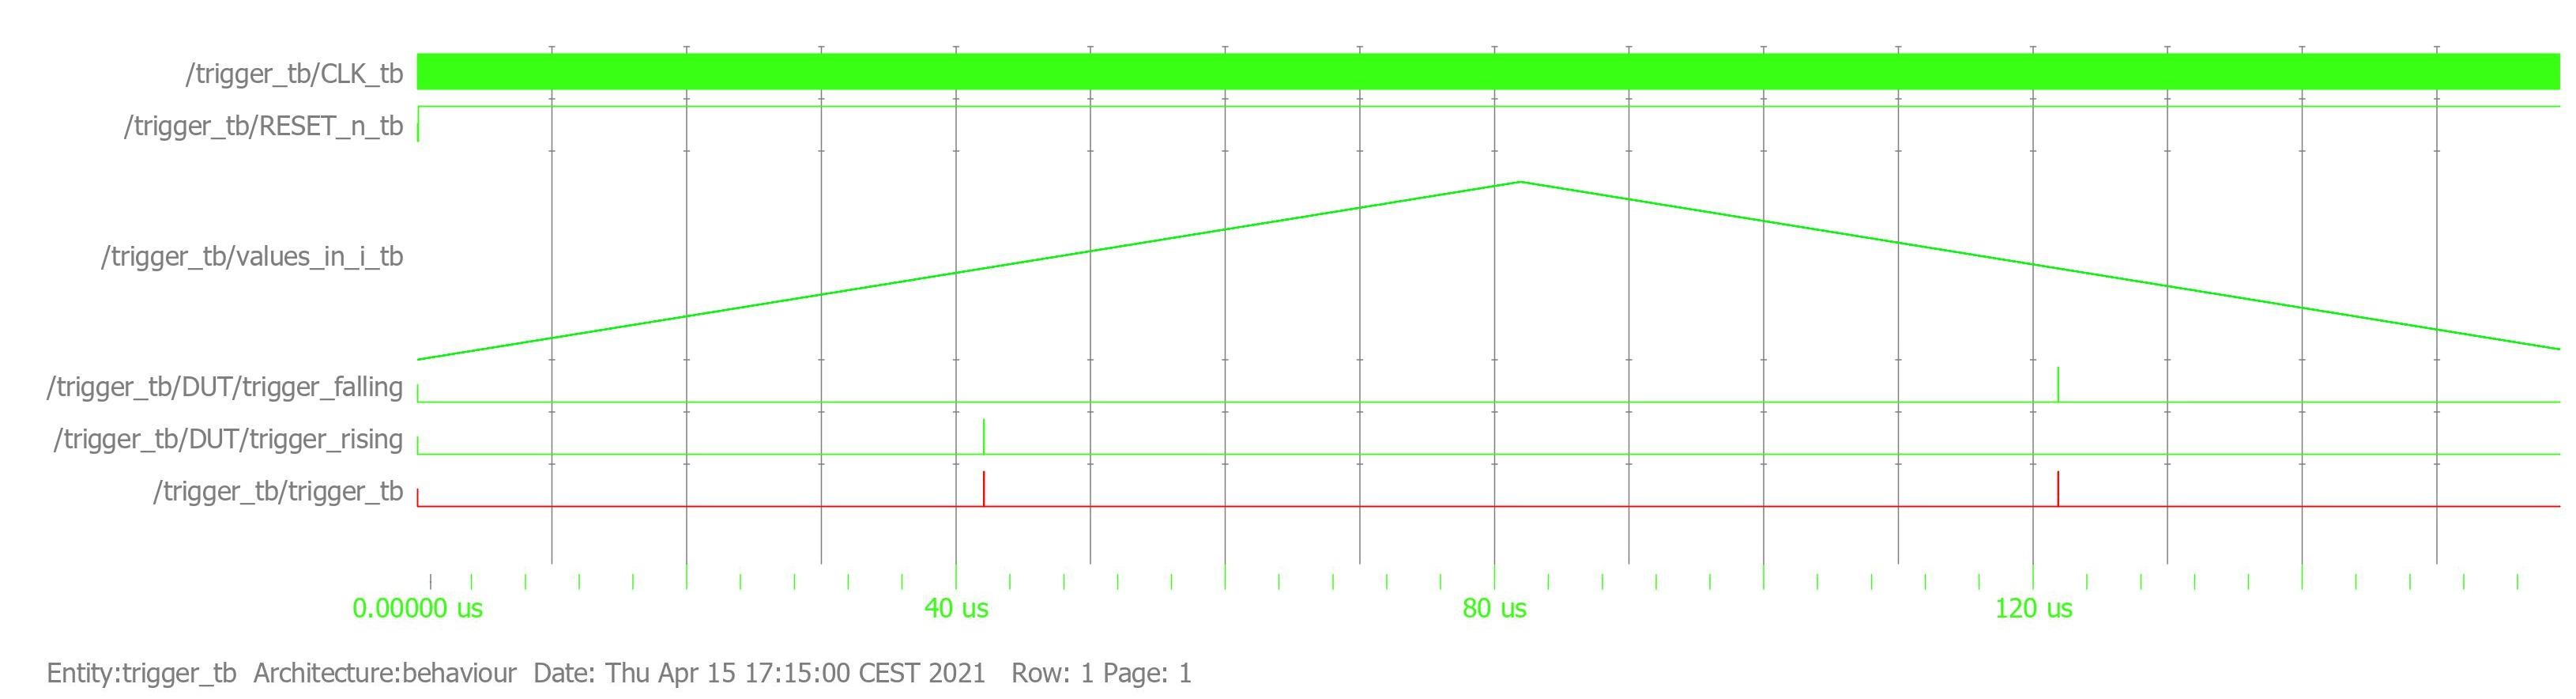
\includegraphics[width=16cm]{SAUER/Grafiken/Trigger/Simulation.jpg}
		\caption{Simulation}
		\label{TriggerSim}
	\end{center}
\end{figure}